\section{Einrichtung der Docker-Infrastruktur}


Zu den Herausforderungen, die von der Testinfrastruktur erwartet
werden, gehören Konzepte wie die vollständige Automatisierung,
die lokale Installation und die \"Ubertragbarkeit der Testwerkzeuge
auf verschiedene Umgebungen. Um diese Erwartungen zu erfüllen,
wurden Werkzeuge wie Docker entwickelt. In diesem Kapitel wird
zunächst eine kurze Beschreibung von Docker gegeben. Anschließend
wird gezeigt, wie Docker bei der Entwicklung der Testinfrastruktur
von jExam eingesetzt wurde, und schließlich werden die Ergebnisse
der Entwicklung vorgestellt.

\subsection{Docker}

Bei der Entwicklung einer Anwendung gibt es einige Probleme, die
sehr oft während der Entwicklung oder sogar während der Produktion
auftreten. Diese Probleme werden oft durch die folgenden Aussage
formuliert:

\begin{enumerate}
    \item Das Skript funktionierte gestern aber heute nicht mehr.
    \item Das Skript funktioniert auf diesem Rechner und nicht auf
    dem Rechner eines Kollegen/Kunden.
    \item Das Skript funktioniert nur mit Java 5 und nicht mit Java 8.
    \item Die Anwendung muss in allen aktuellen Browser-Versionen von Chrome (80,81,82,\ldots,89) und Firefox (78,79,80,\ldots,84) getestet werden.
    Mussen die alle installiert werden ?
\end{enumerate}

Docker ist eine Open-Source-Containerisierungsplattform. Sie
ermöglicht es Entwicklern, Anwendungen in \gls{container}
(standardisierte ausführbare Komponenten) zu verpacken.
Sie kombinieren den Quellcode der Anwendung mit den
Betriebssystembibliotheken und Abhängigkeiten, die für die
Ausführung dieses Codes in jeder Umgebung erforderlich sind.
Container vereinfachen die Bereitstellung verteilter Anwendungen und
erfreuen sich zunehmender Beliebtheit (vgl. \cite{docker}).

Docker macht das Erstellen, Bereitstellen und Verwalten von
Containern leichter, einfacher und sicherer (vgl. \cite{ibm-docker}).
Docker ist im Wesentlichen ein Toolkit, das es Entwicklern ermöglicht,
Container mit einfachen Befehlen und arbeitssparender Automatisierung
über eine einzige API zu erstellen, bereitzustellen, auszuführen,
zu aktualisieren und zu beenden (vgl. \cite{ibm-docker}). Zu den Vorteilen der Verwendung von
Docker gehören :

\begin{itemize}
    \setlength\itemsep{1em}
    \item[] \textbf{Portabilität}: Ein Container erstellt ein ausführbares
    Softwarepaket, das vom Host-Betriebssystem abstrahiert
    (nicht an dieses gebunden oder von diesem abhängig ist)
    und daher portabel und in der Lage ist, auf jeder Plattform oder
    Cloud einheitlich und konsistent zu laufen.

    \item[] \textbf{Agilität}: Docker für die Ausführung von Containern hat den
    Industriestandard für Container mit einfachen Entwicklertools
    und einem universellen Paketierungsansatz geschaffen, der sowohl
    unter Linux- als auch unter Windows-Betriebssystemen funktioniert.
    Das Container-\"Okosystem hat sich auf Engines verlagert, die von
    der Open Container Initiative (OCI) verwaltet werden.
    Softwareentwickler können weiterhin agile oder DevOps-Tools
    und -Prozesse für eine schnelle Anwendungsentwicklung und
    -verbesserung verwenden.

    \item[] \textbf{Geschwindigkeit}: Container werden oft als leichtgewichtig
    bezeichnet, was bedeutet, dass sie den Betriebssystemkern des
    Rechners gemeinsam nutzen und nicht mit diesem zusätzlichen
    Overhead belastet werden. Dies steigert nicht nur die Effizienz
    des Servers, sondern senkt auch die Server- und Lizenzkosten und
    verkürzt die Startzeiten, da das Betriebssystem nicht gebootet
    werden muss.

    \item[] \textbf{Isolierung von Fehlern}: Jede containerisierte Anwendung ist
    isoliert und arbeitet unabhängig von den anderen. Der Ausfall
    eines Containers hat keine Auswirkungen auf den weiteren Betrieb
    der anderen Container. Entwicklungsteams können alle technischen
    Probleme innerhalb eines Containers identifizieren und beheben,
    ohne dass es zu Ausfallzeiten in anderen Containern kommt.
    Außerdem kann die Container-Engine alle
    Sicherheitsisolationstechniken des Betriebssystems nutzen, um Fehler innerhalb der
    Container zu isolieren.

    \item[] \textbf{Effizienz}: Software, die in containerisierten Umgebungen
    ausgeführt wird, teilt sich den Betriebssystemkern des Rechners,
    und Anwendungsschichten innerhalb eines Containers können von
    mehreren Containern gemeinsam genutzt werden. Daher haben
    Container von Natur aus eine geringere Kapazität als eine VM
    und benötigen weniger Anlaufzeit, so dass weitaus mehr Container
    auf der gleichen Rechenkapazität wie eine einzelne VM ausgeführt
    werden können. Dies führt zu einer höheren Server-Effizienz und
    senkt die Server- und Lizenzierungskosten.

    \item[] \textbf{Sicherheit}: Die Isolierung von Anwendungen in Form von
    Containern verhindert von Natur aus, dass bösartiger Code in
    andere Container oder das Hostsystem eindringt. Darüber hinaus
    können Sicherheitsberechtigungen definiert werden, um unerwünschte
    Komponenten automatisch am Eintritt in Container zu hindern oder
    die Kommunikation mit unnötigen Ressourcen einzuschränken.

\end{itemize}


Docker bietet also die Möglichkeit, ein Werkzeug zu bauen, das auf
allen Arten von Systemen unabhängig von den lokalen Konfigurationen
der einzelnen Benutzer funktioniert. Es spielt also keine Rolle,
welche Java-Version oder welches Betriebssystem ein Benutzer hat (vgl. \cite{ibm-docker}).
Anstatt eine Vielzahl von Abhängigkeiten herunterzuladen und zu
installieren, kann man auch einfach einen Container mit allen
notwendigen Abhängigkeiten erstellen und ihn auf jedem System
verwenden, das Docker unterstützt. Die Verwendung von Docker wird all diese Vorteile für die Entwicklung
der Testinfrastruktur nutzen. Das zusätzliche Werkzeug zur
Orchestrierung der verschiedenen Container ist jedoch Docker-compose.


Wenn Sie eine Anwendung aus Prozessen in mehreren Containern erstellen,
die sich alle auf demselben Host befinden, können Sie Docker-Compose
verwenden, um die Anwendungsarchitektur zu verwalten. Docker Compose
erstellt eine YAML-Datei, die die Dienste angibt, die in der Anwendung
enthalten sein sollen, und kann die Container mit einem einzigen
Befehl bereitstellen und ausführen. Mithilfe von Docker Compose ist
es möglich, persistente Volumes für den Speicher zu definieren,
Basisknoten anzugeben und die Abhängigkeiten der Dienste zu
dokumentieren und zu konfigurieren.


Im nächsten Kapitel wird beschrieben, wie Docker und Docker-Compose
für die Einrichtung der Testinfrastruktur von jExam verwendet
wurden.



\subsection{Docker jExam Infrastructur}
Um eine stabile Testinfrastruktur zu schaffen und eine bessere
Verwaltung der Container zu ermöglichen, wurde Docker-Compose
verwendet, um die verschiedenen Testdienste von jExam zu trennen
und zu gruppieren. So kann der Tester nur die Dienste ausführen,
die er braucht und die er testen will. Wenn alle Container
gleichzeitig gestartet würden, könnte dies sehr viele Ressourcen auf
dem Host-Computer beanspruchen und das gesamte System verlangsamen.
Da einige Dienste voneinander abhängig sind, wurde ein Docker-Netzwerk
geschaffen, das die Kommunikation zwischen den ausgeführten Diensten
ermöglicht. Dies ermöglicht ein geschlossenes lokales Netzwerk, das
von außen nicht einsehbar ist (siehe \Cref{fig:dock-net}).

\begin{figure}[H]
    \centering
    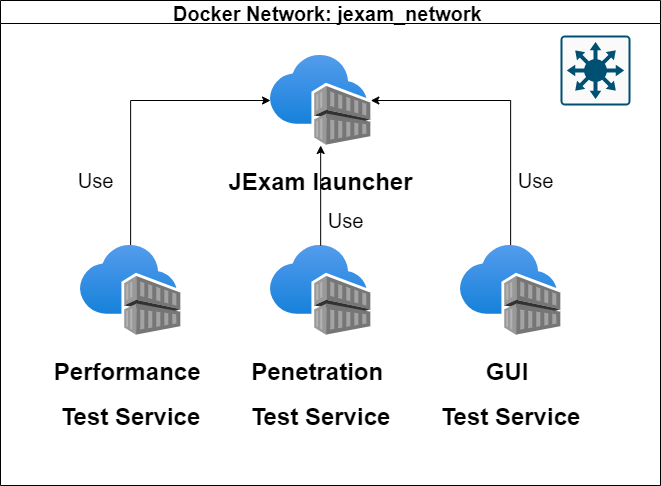
\includegraphics[scale=0.6]{images/all.drawio}
    \caption{jExam Docker Network Darstellung} \label{fig:dock-net}
\end{figure}

\subsubsection{jExam Launcher}

jExam Launcher ist der Hauptdienst der Docker Infrastruktur. Er ist für die Ausführung
und Bereitstellung von \gls{jexam_new} und \gls{jexam_2009} zuständig. Der Dienst
besteht aus fünf Containern, darunter :

\begin{itemize}
    \setlength\itemsep{1em}

    \item[] \textbf{JBoss}: Dieser Container enthält das Skript zum
    Bereitstellen des JBoss-Servers, den \gls{jexam_new} und \gls{jexam_2009}
    benötigen, um funktionieren zu können. Dieser Server dient auch
    als Datenbank für die beiden Apps. Er legt daher einige seiner
    Ports offen, um für externe Verbindungen zugänglich und offen
    zu sein.

    \item[] \textbf{Initializer}: Dieser Container enthält ein
    Java Skript, das automatisch (oder auf Wunsch des Testers auch
    manuell) ausgeführt wird und dazu dient, Testdaten in den 
    JBoss-Server zu injizieren. Es initialisiert die Daten, die für
    die Ausführung der Tests erforderlich sind.

    \item[] \textbf{OldWeb}: Dieser Container ermöglicht das
    Deployment von \gls{jexam_2009}. Er enthält einen Tomcat-Webserver,
    der den Code von \gls{jexam_2009} ausführt und sich dann mit
    dem Container verbindet, der den JBoss-Server enthält.
    Dieser Container legt ebenfalls seine Ports offen, damit er
    von den Tests erreicht werden kann, wenn diese im lokalen 
    Modus ausgeführt werden.

    \item[] \textbf{Webservice und Web}: Diese beiden Container
    ermöglichen die Ausführung und Bereitstellung von
    \gls{jexam_new}. Der Webservice enthält eine API, die vor
    allem mit dem JBoss-Server kommuniziert. Der Web-Container
    enthält das Frontend der Anwendung. Web verbindet sich mit
    dem Webservice, wenn er gestartet wird, und stellt Ports zur
    Verfügung, die ihn zugänglich machen, wenn die Tests im
    lokalen Modus gestartet werden.
\end{itemize}

\begin{figure}[H]
    \centering
    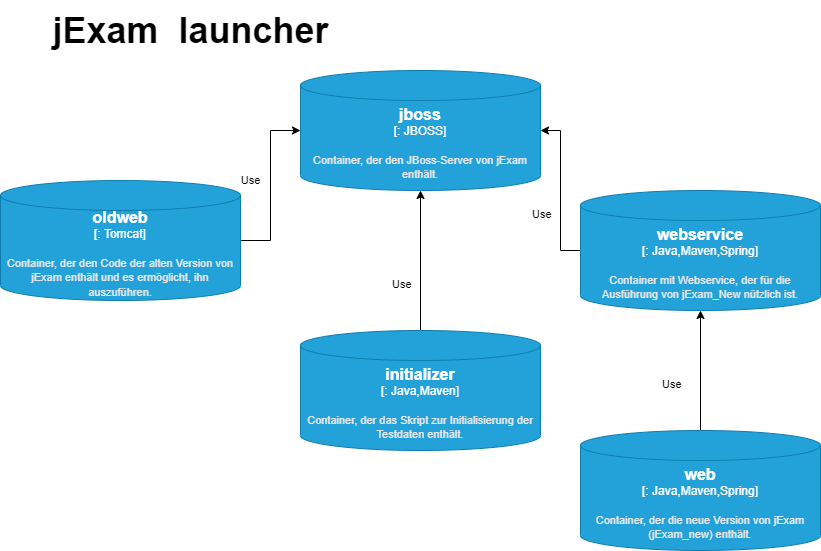
\includegraphics[scale=0.5]{images/launcher.drawio}
    \caption{jExam Launcher Testservice} \label{fig:laucher}
\end{figure}
\subsubsection{UI-Testservice}

Das UI-Testservice ist die Dienststelle, die für die Durchführung
von UI-Tests verantwortlich ist. Es besteht im Wesentlichen aus
vier Containern:

\begin{itemize}
    \setlength\itemsep{1em}

    \item[] \textbf{Selenium-Hub, Chrome- und Firefox-RemoteWebDriver}:
    Der Selenium Hub ist ein Server, der die Zugriffsanfragen vom 
    WebDriver-Client entgegennimmt und die JSON-Testbefehle an die 
    entfernten (remote) Driver weiterleitet. Er nimmt die Befehle vom 
    Client entgegen und führt sie parallel auf den verschiedenen 
    remote Driver aus. Dies ermöglicht die Verwendung der 
    RemoteWebDriver Chrome und Firefox, die direkt mit dem
    Selenium-Hub verbunden sind. Der Tester kann also wählen,
    welchen Browser er für die Ausführung seiner Tests verwenden
    möchte. Es ist jedoch wichtig, darauf hinzuweisen, dass die 
    Container, die die RemoteWebDriver enthalten, so konfiguriert 
    sind, dass sie mit der neuesten Version des Browsers ausgeführt 
    werden, die bei jedem Docker Image Build automatisch 
    heruntergeladen wird.

    \item[] \textbf{UI-Test}: Dieser Container enthält die UI-Tests
    und ist dafür zuständig, diese automatisch mithilfe eines
    Maven-Skripts auszuführen. Wenn die Tests im Remote-Modus
    konfiguriert sind, verbindet sich der Container mit dem
    Selenium-Hub, um Zugriff auf den verfügbaren RemoteWebDriver
    zu erhalten.
\end{itemize}

\begin{figure}[H]
    \centering
    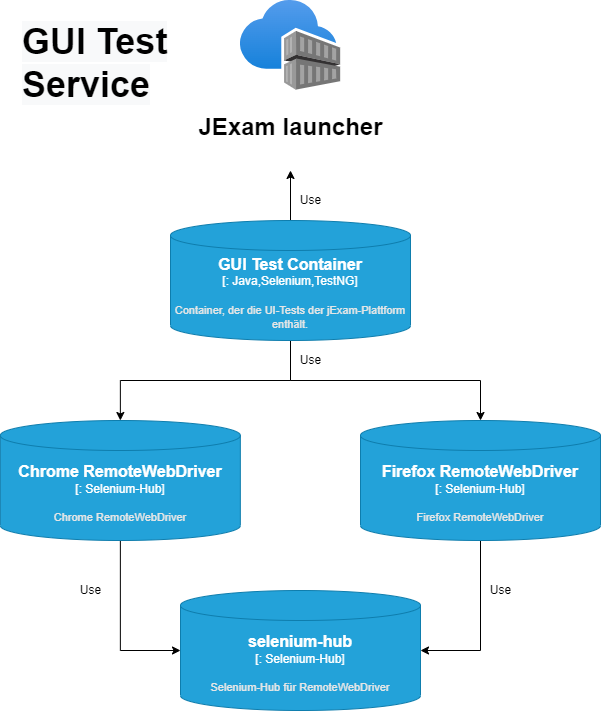
\includegraphics[scale=0.6]{images/gui.drawio}
    \caption{JExam UI Testservice} \label{fig:ui}
\end{figure}
\subsubsection{Penetration Testservice}

Das Penetration Testservice ist der Dienst, der für die Ausführung
von Penetrations- und Sicherheitstestskripten verantwortlich ist.
Dieser Dienst besteht aus einem einzigen Container:

\begin{itemize}
    \setlength\itemsep{1em}

    \item[] \textbf{Owasp}: Dieser Container besteht aus einem
    stabilen Abbild von Zapproxy und enthält die verschiedenen
    Skripte, die auf \Gls{jexam_new} und \Gls{jexam_2009}
    ausgeführt werden: zap-baseline und zap-fullscan.

\end{itemize}

\begin{figure}[H]
    \centering
    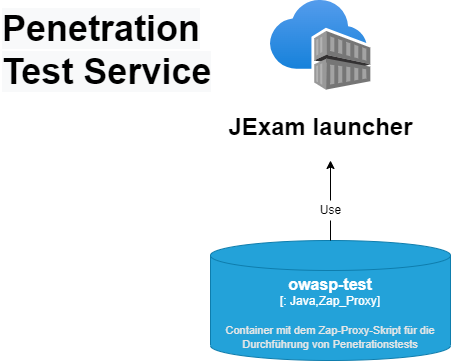
\includegraphics[scale=0.6]{images/penetration.drawio}
    \caption{JExam Penetration Testservice} \label{fig:pen}
\end{figure}


\subsection{Erreichte Ergebnisse}
